\documentclass[12pt]{article}
\usepackage[utf8]{inputenc}
\usepackage[russian]{babel}
\usepackage{graphicx}
\graphicspath{{proteus/}}
\title{Курс молодого бойца}
\author{Ушаков А. Е., Храмцов И. А., Кузнецов В. А.}
\date{\today}
\begin{document}



\maketitle


\newpage
\tableofcontents
\newpage
\section{Необходимый список программ}
\begin{itemize}
\item Atmel Studio 6
\newlineЭто весьма популярная среда программирования для контроллеров Atmel, предоставляется бесплатно.
\newline $http://www.atmel.com/tools/atmelstudio.aspx$
\item ChipProg Usb
\newline Среди оборудования ЛЭМФ есть программатор ChipProg40, способный программировать в параллельном режиме почти любой микроконтроллер. Из-за его устройства наиболее удобно программировать микроконтролеры в DIP корпусе. Сама программа устанавливается и запускается только при наличии подключенного к компьтеру программатора.
\newline $http://www.phyton.ru/download/$
\item Sprint-Layout
\newlineПростой, но в тоже время очень эффективный программный пакет для проектировки и ручной разводки печатных плат малой и средней сложности.
\newline $http://cxem.net/software/sprint\_layout.php$
\item Proteus (для моделирования всего и вся) Ссылку находить на торрентах:)
\end{itemize}
\section{Справочный материал}
\begin{itemize}
\item Atmega8a DataSheet 
\newline $http://www.atmel.com/images/atmel-8159-8-bit-avr-microcontroller-atmega8a\_datasheet.pdf$
\item Г. И. Донов "Применение микроконтроллеров"
\newline Эту книгу можно взять в библиотеке. Будет полезна тем, кто не хочет читать новый материал из даташита выше сразу на английском.
\end{itemize}






\section{Использование программ}
\subsection{Proteus}
После запуска Proteus(isis.exe) должно открыться окно как на рис.~\ref{p1} 


\begin{figure}[h]
\center{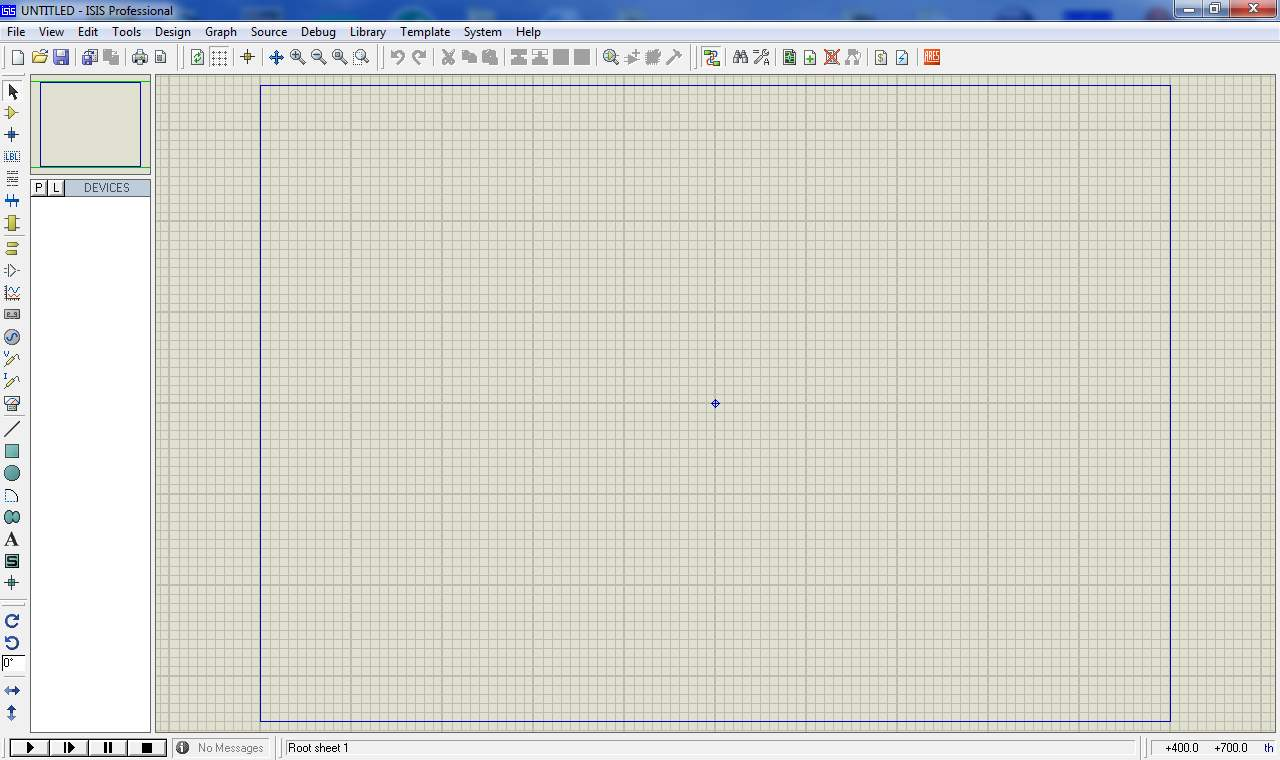
\includegraphics[width=1\linewidth]{1.jpg}}
\caption{Начальное окно Proteus}
\label{p1}
\end{figure}
dffdsg
\section{Куски кода}

\subsection{}
\subsection{}
\subsection{Usart и еже с ним}
\subsection{}
\end{document}
